%! Author = UserHome
%! Date = 02.12.2024

\chapter{Algoritmy založené na DFS}

Táto kapitola sa zaoberá algoritmami, ktoré využívajú prehľadávanie do hĺbky (DFS) na riešenie problémov. Tieto algoritmy postupne skúmajú všetky možné riešenia a využívajú techniky, ako je dopredná kontrola a backtracking, na optimalizáciu procesu hľadania riešení.

\section*{DFS}
\section*{Backtracking}
\section*{Dopredná kontrola}
Domény pre tento problém sú definované tak, že každá kráľovná je reprezentovaná ako premenná, ktorá sa nachádza v konkrétnom riadku šachovnice. Doména tejto premennej je množina možných pozícií, ktoré môže kráľovná zaujať v príslušnom riadku. V prípade 4x4 šachovnice má každá kráľovná na začiatku 4 možné hodnoty (stĺpce od 0 do 3) ako je znázornené na obrázku \ref{fig:forward-checking-zero-step}. Akonáhle sa však jedna z kráľovien umiestni na konkrétnu pozíciu, zvyšné hodnoty v doméne sú zredukované na základe konfliktov s ostatnými kráľovnami ako je znázornené na obrázku \ref{fig:forward-checking-first-step}.\par

Ak po umiestnení ďalšej dámy existuje aspoň jeden riadok, do ktorého nie je možné umiestniť dámu bez konfliktu ako je znázornené na obrázku~\ref{fig:forward-checking-empty-domain}, potom sa ďalšia dáma neumiestni a algoritmus vykoná krok späť .


\begin{figure}
    \centering
    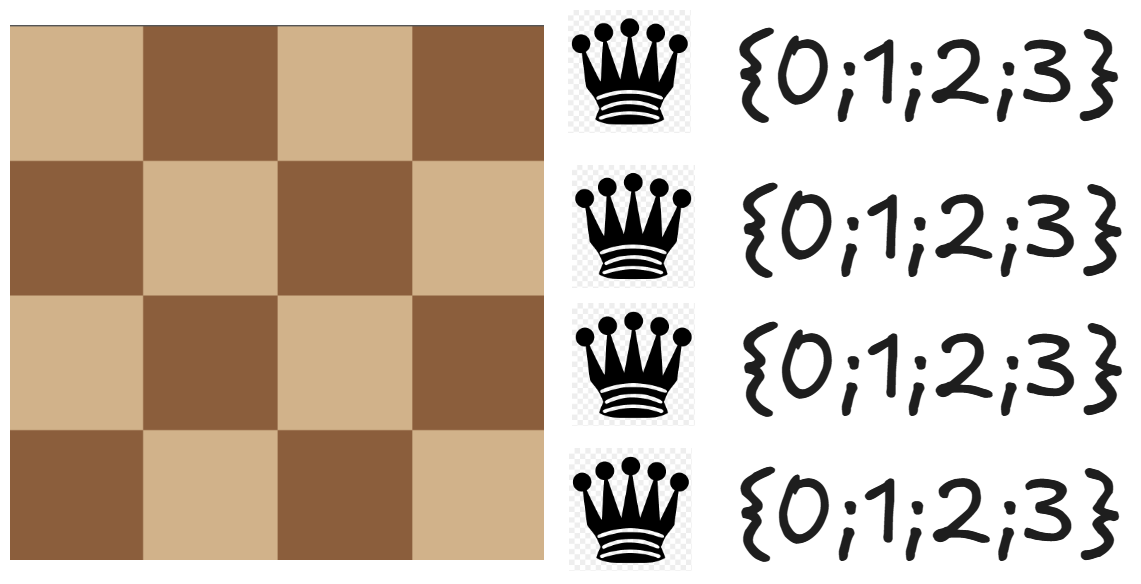
\includegraphics[width=0.7\textwidth]{figs/forward-checking/forward-checking-zero-step}
    \caption{Počiatočný stav doprednej kontroly}
    \label{fig:forward-checking-zero-step}
\end{figure}
\begin{figure}
    \centering
    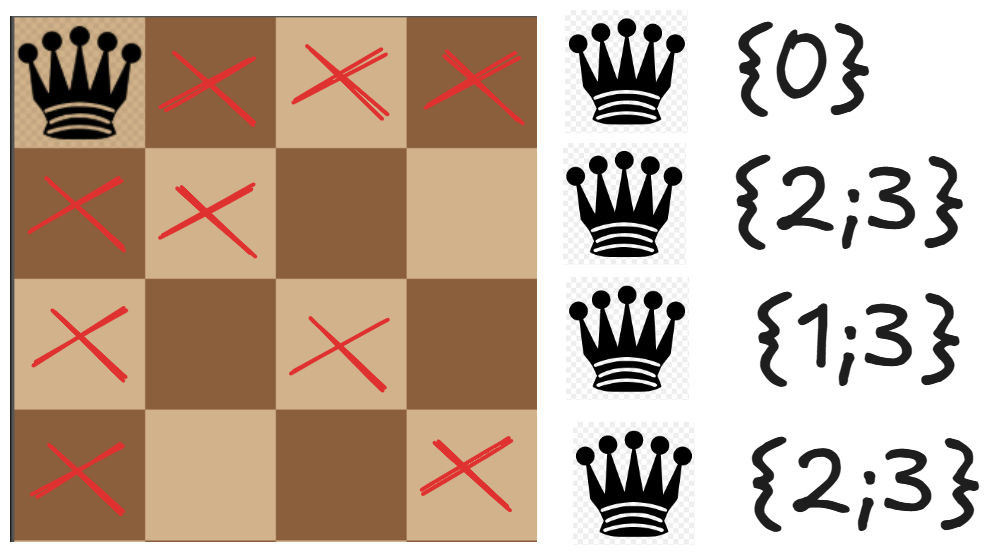
\includegraphics[width=0.6\textwidth]{figs/forward-checking/forward-checking-first-step}
    \caption{Prvý krok doprednej kontroly}
    \label{fig:forward-checking-first-step}
\end{figure}
\begin{figure}
    \centering
    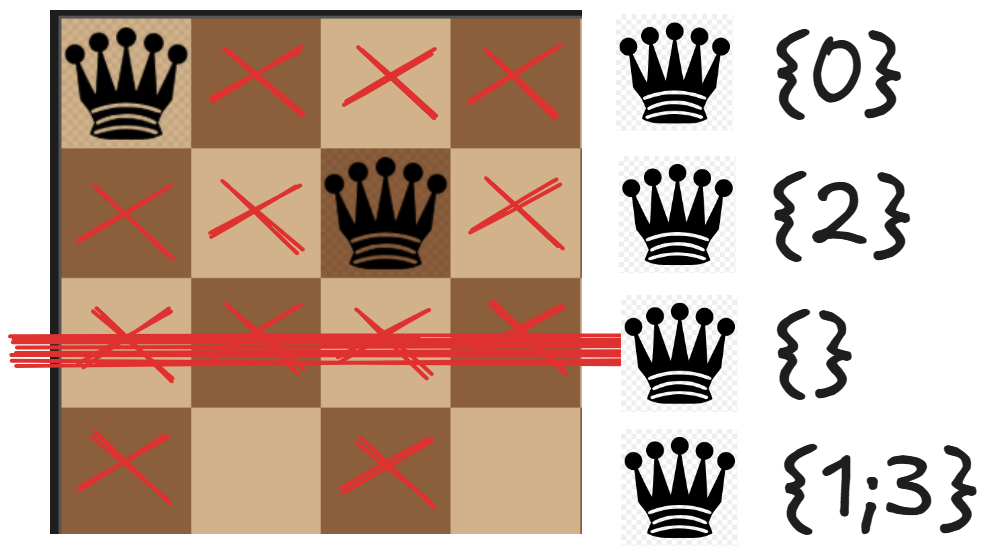
\includegraphics[width=0.6\textwidth]{figs/forward-checking/forward-checking-empty-domain}
    \caption{Prázdna doména v doprednej kontrole}
    \label{fig:forward-checking-empty-domain}
\end{figure}

\subsection{MRV v doprednej kontrola}
Riadok, v ktorom bude umiestnená ďalšia dáma, sa vyberie ako riadok, v ktorom má dáma najmenší počet možných pozícií. Ako je znázornené na obrázku \ref{fig:forward-checking-mrv} prvý riadok\footnote{Číslovanie začína od 0.} má najmenší počet možností umiestnenia kráľovnej, takže kráľovná bude umiestnená na ňom.
\begin{figure}
    \centering
    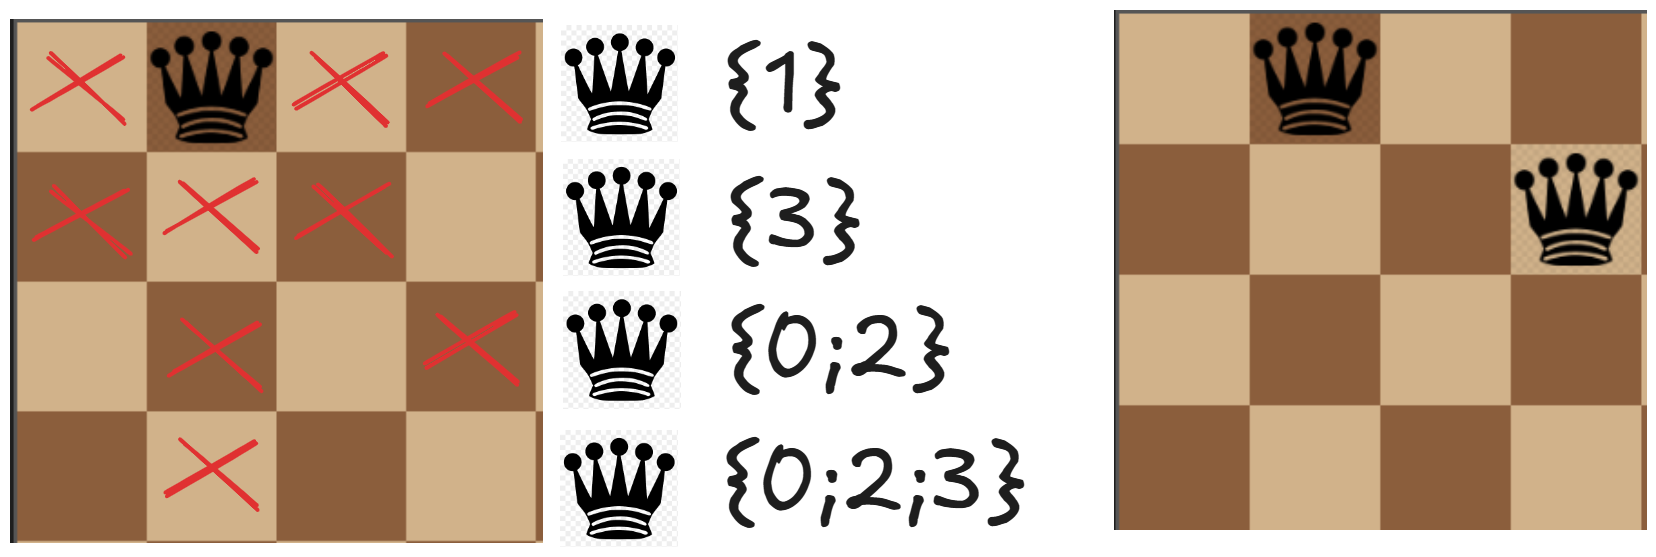
\includegraphics[width=1\textwidth]{figs/forward-checking/forward-checking-mrv}
    \caption{Výber riadku pri doprednej kontrole pomocou MRV}
    \label{fig:forward-checking-mrv}
\end{figure}

\subsection{LCV v doprednej kontrola}
Po výbere riadku pomocou MRV sa vyberie stĺpec, v ktorom bude umiestnená kráľovná. Vyberie sa pozícia, na ktorej kráľovná vytvorí najmenší možný počet nových konfliktov. Na obrázku \ref{fig:forward-checking-lcv} prvá kráľovná vytvorí 2 nové konflikty a druhá vytvorí 3 konflikty.
\begin{figure}
    \centering
    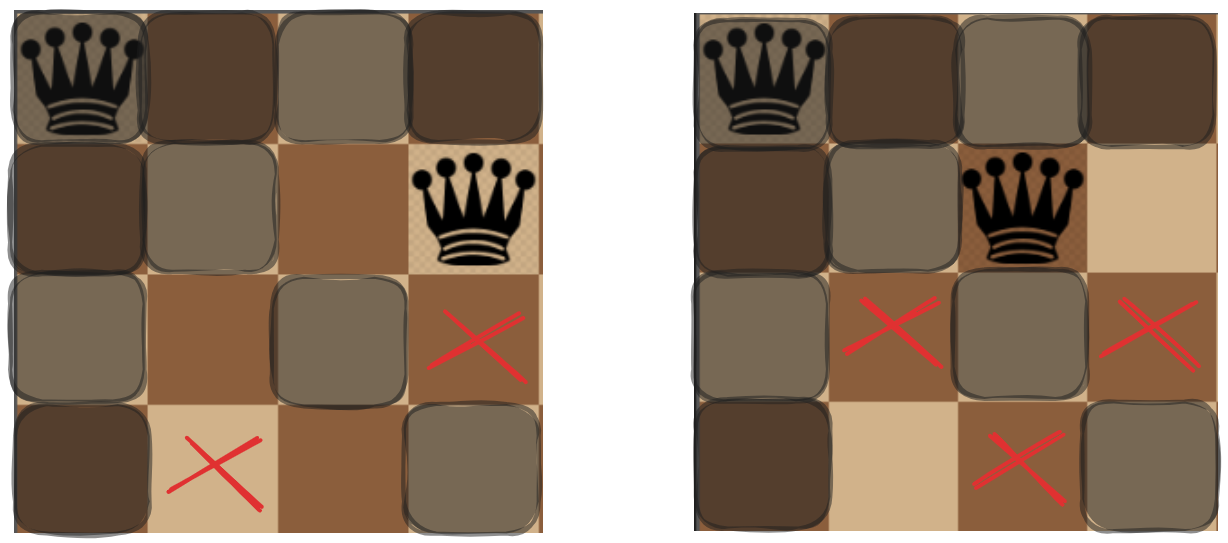
\includegraphics[width=0.8\textwidth]{figs/forward-checking/forward-checking-lcv}
    \caption{Výber stĺpca pri doprednej kontrole pomocou LCV}
    \label{fig:forward-checking-lcv}
\end{figure}
